\section{Les sociétés de contrôle}

\paragraph{Une portée personnelle}

\paragraph{} L'utilisation d'un service est de nos jours synonyme de production et donc collecte de données ; ne dit-on
pas que si un service est gratuit, c'est que ses utilisateurs en sont les produits ? Dès lors nous ne sommes plus maîtres
des informations que nous publions, qui peuvent être vendues ou récupérées à des fins diverses : publicité et marketing
ciblés en sont des exemples bien connus.

\paragraph{} Mais les données ne sont pas uniquement utilisées de manière ciblée. Le développement ces dernières années 
des \emph{Smart Cities} donne naissance à des initiatives impensables auparavant. Ainsi la ville de New York s'est-elle
dôtée d'un tableau de bord \cite{ProgrammableCity1} aggrégeant l'ensemble des sources de données à sa disposition pour 
mettre en exergue de nombreux indicateurs : fluctuation du prix de l'immobilier, évolutions du nombre de plaintes pour 
tapage nocturne par quartier, niveau de saleté dans les rues, état de la circulation aux différentes heures de la 
journée... Toutes ces données dont \emph{nous} sommes la source sont ainsi mises au service de la ville.

\paragraph{} \emph{The Programmable City} \cite{ProgrammableCity0} est un projet proposant de mettre la technologie au
service de l'urbanisme. Une infrastructure et un ensemble de programmes nous permettent de piloter et d'être à l'écoute
de la ville, qui bénéficie au quotidien d'une attention nouvelle : on crée alors un cercle vertueux. Le site
\url{http://DublinDashboard.ie/} est une mise en application de ces concepts pour la ville de Dublin, proposant des
dizaines de sources de données visualisables concernant l'agglomération. D'autres initiatives, comme celle de SideWalk Labs
à Toronto \cite{ProgrammableCity3}, visent à réinventer la ville pour remettre l'humain au c\oe{}ur des processus de
décision en utilisant les nouvelles technologies et les données générées pour améliorer de manière continue les services
qu'elle fournit.

\begin{figure}[h]
    \centering
    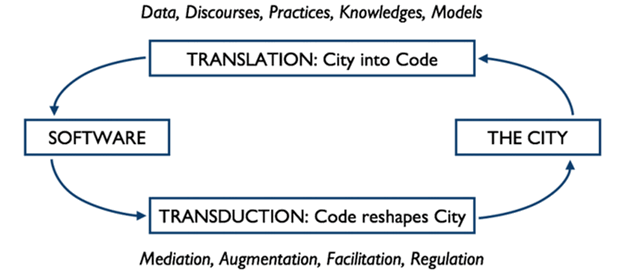
\includegraphics[width=300px]{chapters/01/images/programmable_city.png}
    \caption{\label{programmable_city} Le cycle de transduction des \emph{Programmable Cities}}
\end{figure}

\paragraph{} Une donnée, ce n'est rien de plus que de l'information numérisée. Là où ces bases de données publiques
émanant de structures privées ne nous étonnent en rien - car nous sommes \emph{habitués} à les alimenter, comme l'application
Uber Movement permettant d'analyser les trajets effectués via le service Uber -, il est important de comprendre
qu'elles ne diffèrent pas de celles de nos services publics. Ce n'est qu'avec l'adoption progressive de l'\emph{Open
Data} que ces derniers se sont petit à petit ouverts au développement d'applications exploitant toutes sortes de données. 

\paragraph{} Bien évidemment, les \emph{Open Data} et autres sources de données des \emph{Smart Cities} ne sont pas
constituées de données personnelles - c'est à dire d'informations permettant d'identifier de manière directe ou non une 
personne physique \cite{PersonalData0}. Mais cela est-il réellement différent ? Ainsi la société Hitachi a-t-elle développé
en 2015 un système de détection des crimes reposant sur du machine learning \cite{ProgrammableCity2}. Une quantité
astronomique de données de toutes sortes est nécessaire pour alimenter le système, des mouvements de population aux 
antécédents de crimes enregistrés dans les zones sous surveillance. Ne peut-on pas alors craindre de voir une zone 
démographique désertée suite à un incident car son \emph{coefficient de criminalité} aura augmenté, rebutant nouveaux
résidents et jeunes parents à s'y installer ?

\paragraph{} Se savoir surveillé restreint-il les instincts pervers ?
Ou au contraire cela les désinhibe-t-il ? Il convient avant tout de définir ce que l'on
entend par \emph{instinct}. La surveillance peut-elle vraiment anéantir toute perversion ?
Parallèle possible avec les radars routiers automatiques : ont-ils fait disparaitre les
infractions par excès de vitesse ? Le poblème de la perversion est qu'elle fait partie
intégrante de nous-même, quelle qu'elle soit. Vaudrait-il mieux alors vivre dans une société
où sévissent une dizaine d'êtres extrêmement pervers, ou dans une société où la perversion
est \emph{lissée}, \emph{amortie}, \emph{normalisée}, présente chez tous à un degré infime...
mais toujours présente ? La prévision (d'un crime, par exemple), amènerait-elle à changer
son comportement ? Panoptique, surveilleur-surveillé. 


\paragraph{Évolution du partage}

\paragraph{} Évolution du partage : les réseaux sociaux, quelles moeurs ? Catégoriees d'âges ? Sociaux-professionnelles ?
Quelle forme de contrôle incarnée par notre prototype ? À qui est-il destiné ? Pour quelles utilisations ?
La place de l'information/désinformation ?


\paragraph{L'individu technique}

\paragraph{} Comment les modèles de sociétés nous ont-ils amené à réfléchir l'individu en termes technologiques ?